\documentclass[12pt, a4paper, oneside]{article}\usepackage[]{graphicx}\usepackage[]{color}
%% maxwidth is the original width if it is less than linewidth
%% otherwise use linewidth (to make sure the graphics do not exceed the margin)
\makeatletter
\def\maxwidth{ %
  \ifdim\Gin@nat@width>\linewidth
    \linewidth
  \else
    \Gin@nat@width
  \fi
}
\makeatother

\definecolor{fgcolor}{rgb}{0.345, 0.345, 0.345}
\newcommand{\hlnum}[1]{\textcolor[rgb]{0.686,0.059,0.569}{#1}}%
\newcommand{\hlstr}[1]{\textcolor[rgb]{0.192,0.494,0.8}{#1}}%
\newcommand{\hlcom}[1]{\textcolor[rgb]{0.678,0.584,0.686}{\textit{#1}}}%
\newcommand{\hlopt}[1]{\textcolor[rgb]{0,0,0}{#1}}%
\newcommand{\hlstd}[1]{\textcolor[rgb]{0.345,0.345,0.345}{#1}}%
\newcommand{\hlkwa}[1]{\textcolor[rgb]{0.161,0.373,0.58}{\textbf{#1}}}%
\newcommand{\hlkwb}[1]{\textcolor[rgb]{0.69,0.353,0.396}{#1}}%
\newcommand{\hlkwc}[1]{\textcolor[rgb]{0.333,0.667,0.333}{#1}}%
\newcommand{\hlkwd}[1]{\textcolor[rgb]{0.737,0.353,0.396}{\textbf{#1}}}%

\usepackage{framed}
\makeatletter
\newenvironment{kframe}{%
 \def\at@end@of@kframe{}%
 \ifinner\ifhmode%
  \def\at@end@of@kframe{\end{minipage}}%
  \begin{minipage}{\columnwidth}%
 \fi\fi%
 \def\FrameCommand##1{\hskip\@totalleftmargin \hskip-\fboxsep
 \colorbox{shadecolor}{##1}\hskip-\fboxsep
     % There is no \\@totalrightmargin, so:
     \hskip-\linewidth \hskip-\@totalleftmargin \hskip\columnwidth}%
 \MakeFramed {\advance\hsize-\width
   \@totalleftmargin\z@ \linewidth\hsize
   \@setminipage}}%
 {\par\unskip\endMakeFramed%
 \at@end@of@kframe}
\makeatother

\definecolor{shadecolor}{rgb}{.97, .97, .97}
\definecolor{messagecolor}{rgb}{0, 0, 0}
\definecolor{warningcolor}{rgb}{1, 0, 1}
\definecolor{errorcolor}{rgb}{1, 0, 0}
\newenvironment{knitrout}{}{} % an empty environment to be redefined in TeX

\usepackage{alltt} % Paper size, default font size and one-sided paper
\usepackage{float}
%\usepackage[dcucite]{harvard}
\usepackage{tikz}
%\usetikzlibrary{shapes, shadows, arrows}
\usepackage{rotating}
\usepackage{amsmath}
%\usepackage{setspace}
\usepackage{pdflscape}
\usepackage[flushleft]{threeparttable}
\usepackage{multirow}
\usepackage[comma, sort&compress]{natbib}% Use the natbib reference package - read up on this to edit the reference style; if you want text (e.g. Smith et al., 2012) for the in-text references (instead of numbers), remove 'numbers' 
\usepackage{graphicx}
\graphicspath{{./Figures/}} % Specifies the directory where pictures are stored
%\bibliographystyle{plainnat}
%\usepackage{listings}
\bibliographystyle{agsm}
\usepackage[colorlinks = true, citecolor = blue, linkcolor = blue]{hyperref}
%\hypersetup{urlcolor=blue, colorlinks=true} % Colors hyperlinks in blue - change to black if annoying
\IfFileExists{upquote.sty}{\usepackage{upquote}}{}
\begin{document}
%\renewcommand[\harvardurl]{URL: \url}
\title{The Forward-Discount Puzzle in Central and Eastern Europe}

\maketitle
\begin{abstract}
This paper adds to evidence that the forward-discount puzzle is at least in part explained as a compensation for taking crash-risk. A number of Central and Eastern European exchange rates are compared. A Hidden Markov Model is used to identify two regimes for most of the exchange rates.  These two regimes can be characterised as being either periods of stability or periods of instability. The level of international risk aversion and changes in US interest rates affect the probability of switching from one regime to the other. This model is then used to assess the way that these two factors affect the probability of a currency crisis. While the Czech Republic,  Hungary and Bulgaria are very sensitive to international financial conditions, Poland and Romania are relatively immune.  

\emph{JEL classifications:} C24, F31, F32; 
\emph{Key words:} Exchange rates, uncovered interest parity, foreign exchange risk discount, hidden-Markov model, carry-trade


\end{abstract}

\section{Introduction}
The common observation that exchange rate changes deviate systematically from the forward rate so that excess returns are available from borrowing low interest rate or funding currency for an investment in higher rate units or the investment currency is called the forward discount puzzle.   This paper uses a two-regime model to understand more about crash-risk by assessing Uncovered Interest Parity (UIP) deviations in a range of CEE countries and by using a Hidden Markov Model (HMM) to divide the deviations into two categories: those where the high-yield currency does not depreciate (or may even appreciate) against the lower interest rate unit and those where the high-yield currency falls much more than would be anticipated by UIP.  In the first case, the conditions are favourable for inflow of capital to the higher interest rate unit.  It would be possible to make profitable carry-trades where funds are borrowed in the lower rate unit currency, transferred into the currency with the higher interest rate for the same period as the borrowing and then exchange back and repaid at the end of the contract. These are likely to be times of relative calm in the foreign exchange market. In the second case, these carry-trades would be more likely to lose money and a sharp depreciation of the high yield currency would be likely to be associated with exchange rate crisis. 

The first regime might be called the period of 'calm' and is a much more common occurrence. The second period is rare and could be called 'crisis'.  We use a Hidden Markov Model to estimate the probability of switching from a calm regime to one of crisis for each country and to assess the way that these probabilities are affected by exogenous events such as international risk aversion and changes in US interest rates.  These exogenous factors increase the risk of experiencing an exchange rate crisis and can be used to compare how vulnerable each country is to these type of external shocks. 



This paper adds to the evidence that the forward discount puzzle is explained as a compensation for taking crash-risk, builds on the use of non-linear methods  and greatly extends and expands on the use of HMM models for understanding the forward discount puzzle.  This paper also contributes to the literature on \emph{sudden stops} as it provides for comparative measures of the probability that a period of calm in the foreign exchange market will switch to one of crisis and it also measures how this probability is affected by changes in international risk appetite and changes in US interest rates.  The rest of this paper proceeds as follows, Section 2 discusses the forward discount puzzle, Section 3 presents the Hidden Markov Model, Section 4 analyses the initial results, Section 5 considers exogenous influences on the probability of switching from one regime to another and Section 6 concludes. 
%What is the research gap?  How does the paper contribute to the literature. 

\section{Literature}
 \label{secref:UIP}
The forward rate today is the rate that currencies can be exchanged in the future.  Covered Interest Parity (CIP) asserts that, given the free flow of international capital and competitive markets,  the difference between the spot rate and the forward rate must be equal to the interest rate differential for the two currencies for the same period.    

\begin{equation}
\frac{F_{t, j}}{S_t} \times (1 + i_{t,j}^*) = (1 + i_{t,j})  
\end{equation}

where $F_{t, j}$ is the forward exchange rate at time t for domestic currency in terms of overseas for j periods ahead;  $S_t$ is spot exchange rate under the same terms at time t; $i_{t,j}$ is the interest rate for the home currency in period t for j periods ahead; $i_{t, j}^*$ is the interest rate for the overseas currency at time t for j periods ahead.

Therefore, 

\begin{equation}
\frac{F_{t,j}}{S_t} = \frac{(1 + i_{t, j})}{(1 + i_{t, j}^*)} 
\end{equation}

 Re-arranging

\begin{equation}
\label{eq:fw}
\frac{F_{t,j} - S_t}{S_t} = \frac{(i_{t,j} - i_{t,j}^*)}{(1 + i_{t,j}^*)} 
 \end{equation}

Assuming rational expectations and no financial frictions, the forward rate should be the best unbiased estimate of the future spot rate and therefore, Equation \ref{eq:fw} becomes.  

\begin{equation}
\frac{E[S_{t+j}] - S_t}{S_t} = \frac{(i_{t, j} - i_{t, j}^*)}{(1 + i_{t, j}^*)}
\label{eq:UIP1}
\end{equation} 

if $i^*$ is relatively small, this can be approximated by 

\begin{equation}
E[s_{t+j}] - s_t = i_{t,j} - i_{t,j}^* 
\end{equation} 

where $s_t$ is the log of the exchange rate at time t, $s_{t + j}$ is the log of the exchange rate at t plus j, $i_{t, j}$ is the j-period interest rate at time t and $^*i_{t, j}$ is the the foreign currency j-period interest rate at time t.  

Assuming that CIP holds\footnote{Since the global financial crisis there is increased evidence that this is not the case as credit and regulatory frictions have become more prominent.} so that the forward rate can account for the interest rate differential, a test of UIP can take the form of 

\begin{equation}
\label{eq:uip2}
\Delta s_{t + j} = \beta_0 +\beta_1 f_{t+j} + \varepsilon
\end{equation} 

where $\Delta s_{t + j}$ is the change in the log of the exchange rate between period t and j, $f_{t+j}$ is the forward discount expressed as the difference between the logs of the spot rate and the forward rate for $j$ periods ahead of $t$; $\varepsilon$ is an error term, while $\beta_0$ and $\beta_1$ are the coefficients to be estimated.  If UIP holds, $\beta_0$ should be equal to zero and $\beta_1$ should be equal to one as again the forward rate should be an unbiased estimate of the future exchange rate.   

However, this standard test of UIP consistently finds that estimates of  $\beta_1$ are less than one.  A meta-study by \citet{FrootUIP} found that the 75 published estimates had an average value of -0.88 for $\beta_1$.   An investment that takes advantage of this deviation by borrowing the low interest rate funding currency for a deposit in the higher interest rate investment currency is called \emph{the carry-trade}.  The evidence that the carry-trade is profitable is consistent with the forward discount puzzle.  
%need further and more recent evidence here. this may be the place for the evidence and an expansion of the next paragraph.  

As UIP is a key component of international financial theory, there has been a tremendous effort to understand this \emph{puzzle}.  See \citet{FrootUIP}, \citet{Hodrick1987},  \citet{Engel1996} and \citet{EngelHandbook} for a summary of the vast literature in this area. Some suggest that it is the lack of stationarity in the series that causes estimation problems.  \citet{Engel1996} and \citet{Roll2000}; others argue that this is really an issue for developed rather than developing nations \citet{Bansal1999};  tests using 10 year bond yields indicate that the puzzle applies to the short-term but not long-term rates.  See \citet{Chinn2004} for example.  It may also be associated with factors like heterogeneous market agents or asymmetry of information. See \citet{Bacchetta2012} for a survey of contributions in this area. There is also a wide ranging discussion over whether, once the assumption of risk-neutrality is abandoned, the apparent breakdown is the result of failing to correctly account for this risk. The last of these is explored here. 

\subsection{Risk premium}
If investors are risk averse and form their expectations rationally, the negative estimate for $\beta$ could mean that investors required additional return for holding foreign currency assets and Equation \ref{eq:uip2} can be augmented with a term that would account for this \emph{risk premium.}  

\begin{equation}
\label{eqref:fb1}
E[\Delta s_{t + j}]= \beta_0 +\beta_1 f_{t+j} + \beta_2 rp^{re}_{t +j} + \varepsilon
\end{equation}

where $rp^{re}_{t, j}$ is a rational expectations risk premium at time $t$ for $j$ periods ahead.  This seemed reasonable for the original US-centric research but it means that none US residents require a risk premium for investing at home.   \citet{CanovaMarrinan} find that this risk premium switches from positive to negative as relative interest rates change and that the risk premium has a large variance, serial correlation and has volatility clustering.  \citet{FamaUIP} finds that the variation in the risk premium is much larger than the variation in the exchange rate or the forward rate and that there is a negative correlation between the premium and the expected spot rate.    \citet{FrootUIP} discovers that short rates consistently predict excess returns even outside currency markets.  For foreign exchange, stock, bond and commodity markets, a one percentage annualised increase in the short-term interest rate is associated with about a three percentage point reduction in annualised excess returns. This all seems to undermine the simple risk premium approach to the forward discount puzzle. 

\citet{Engel1996} has identified that this risk premium only holds under rational expectations. Market expectations may differ from the information that is used to test Equation \ref{eq:uip2}. This divergence in expectations can be divided into two types: where the econometrician has more information that the agent (the agent gradually learns the model as was the case when floating exchange rates returned in 1973) or where the agent has information that the econometrican does not have (there may be peso problems where a large depreciation is anticipated that has not previously been recorded in the data).  In each of these situations we could expect the asymmetry to dissipate over time as agents learn and the data becomes available. This has not happened. 

Another avenue of enquiry will seek support for the risk premium approach and explanation for its volatility by looking for a relationship with common risk factors.  \citet{Burnside2010} assess whether carry-returns are correlated with conventional risk factors like the equity risk-premium or real consumption growth and volatility indices.  They find limited correlation. \citet{McCallum} assumes that $rp^{re}$ is a stochastic process and asks whether there are reasonable grounds for this to be negatively correlated with $E(s_{t+1}-s_t)$ as is found empirically.  He concludes that this residual represents all the other factors that are not in the model rather than a risk premium.   

\citet[p.148]{Engel1996} says that $rp^{re}$ could represent `expected profit opportunities` As has been seen, these expected profit opportunities are large and highly variable.  There are a number of studies that have assessed the skewed nature of the returns that are associated with the carry-trade.  These explanations are usually grouped under the term \emph{crash-risk}.  \citet{BrunnermeierCarry} develop a general model of \emph{crash risk}, which is due to the sudden unwinding of the carry trade.  The crash happens when risk-appetite and funding-liquidity decrease and carry positions are swiftly unwound. A potential carry-trade is calculated 

\begin{equation}\label{eqref:carry}
z_{t+1} \equiv (i^* - i) -\Delta s_{t+1}
\end{equation}

where $z_{t+1}$ is the return in excess of the prediction of UIP as $i^*$ is the overseas three  month interest rate and $i$ is the domestic three month interest rate and $\Delta s_{s+1}$ is the change in the log of the exchange rate measured as foreign currency per US dollar \citet[pp. 8-9]{BrunnermeierCarry}.   They find that carry trades have large Sharpe Ratios, negative skewness and positive excess kurtosis.  

\citet{BrunnermeierLiquidity} show how this \emph{crash risk} can be caused by the interaction of illiquidity, margin calls and the evaporation of funding for speculation.  When conditions deteriorate, investors seek to exit the carry position, liquidity declines, banks become more cautious about funding speculative positions and an increase in margin requirements together with a reduction in funding lead to spirals of selling and exaggerated price movements.

 \citet{SpronkEER} augment a traditional heterogeneous agent model with carry traders in addition to fundamental and chartist traders.  Traders adjust their strategy towards those that are most successful. The carry trade is built while conditions are calm.    The model is able to replicate the heavy tails, excess volatility and volatility clustering that is evident in foreign exchange returns.  

\citet{Jurek2} tries to quantify the crash risk by using out-of-the-money put options to hedge the risk of a sharp depreciation of the investment currency.  By comparing the performance of hedged and un-hedged positions, he finds that less than one third of carry-trade excess returns can be explained by crash risk.   \citet{Burnside2010} use a similar method and find similar results.  However, the focus in each of these cases is G20 with only Australia, New Zealand, South Africa and Norway among the traditional carry-trade countries.  The variability of funding and the changes in liquidity are likely to be much greater in emerging economies. \citet{Hayward2014} investigated Central and Eastern European exchange rates and find that during periods of high international risk aversion the carry-trade experiences much lower returns and returns that are characterised by large-skew and kurtosis.  It appears that the returns that are available under normal or calm conditions are a compensation for taking the risk of large losses when risk aversion rises and liquidity disappears. Carry-trade profits and the break down in UIP only seem to happen during the calm period. 

\section{The Hidden Markov Model}\label{secref:HMM}
  A Markov process depends only on the previous state.  A Markov model describes the probability of moving from one set of states to another.  Markov models have been used to understand a wide range of phenomena from weather forecasting, speech recognition and internet search.  If the states that are to be explained can be observed, the probability of being in a particular state and the probability that there is a switch from one state to another can be estimated from a sample.  However, in many cases the states cannot be observed and then the states as well as the transition probabilities must be estimated from the data with a \emph{Hidden Markov Model} (HMM).   

\citet{hamilton1988rational} used a HMM to incorporate discrete changes in expectations about Fed policy to improve the match between the expectations theory and the term structure of interest rates.  This technique assumes that there are unobserved market-expectation regimes and that the adjustment from one state to another is governed by a set of probabilities.  \citet{Hamilton1989} also analysed the performance of postwar US GNP with adjustments from periods that are termed recessions to those that are called expansions. The parameters of an ARIMA representation of US GNP shift between the two regimes so that in periods of recession the underlying growth rate is three percentage points lower than it is during the expansionary period.   

\citet{schaller1997regime} used the same method to assess stock returns in two regimes, uncovering strong evidence of regime-switching between bull and bear markets in the mean and variance of US stock returns.  They also find that that the response of stock returns to the price-dividend ratio is asymmetric as adjustment is much swifter during the bull market phase; \citet{dueker1997markov} employ a HMM so that switches from periods of low to high volatility explain the evolution of US equities from calm conditions to those that are more like a crisis.

\citet{Elliot} use a HMM for the forward discount. They find evidence against UIP and suggest that a three regime model fits the data most effectively.  However, the study only assesses the GBP-USD exchange rate and other factors that may affect the transition probabilities are not considered.  We aim to analyse potential carry-trade profits as arising from one or more regimes.  

\subsubsection{The model}
The first step is to determine whether a one, two or three regime model is the most appropriate.  A  model with more than one regime is often called a \emph{mixture model} as the population of potential carry-trade returns are assumed to come from two or more unobserved sub-populations.  
 In this case, the carry-trade returns are observable and are used to identify the underlying exchange rate.  

Figure \ref{figref:HMM2} gives an overview of the system.  The HMM has three components: $\pi, A, B$:

\begin{itemize}
\item the prior model: $P(S_1 = n| \theta_{prior})$ $(\pi)$
\item the transition model: $P(S_t| S_{t-1}, \theta_{trans})$ $(A)$
\item the response model: $P(Y_t| S_t, \theta_{resp})$ $(B)$
\end{itemize}

There are $n$ states or regimes; $Y_t$ are the observed carry-trade returns; and $\theta_{prior}$, $\theta_{trans}$ and  $\theta_{resp}$ are the parameters of the prior, transition and response models respectively. The unobserved financial regimes are modelled as a Markov chain that determines the probability of switching between two regimes.  The carry-trade returns are affected by the underlying regime and are used to estimate the probability of being in a particular regime.    


\begin{figure}
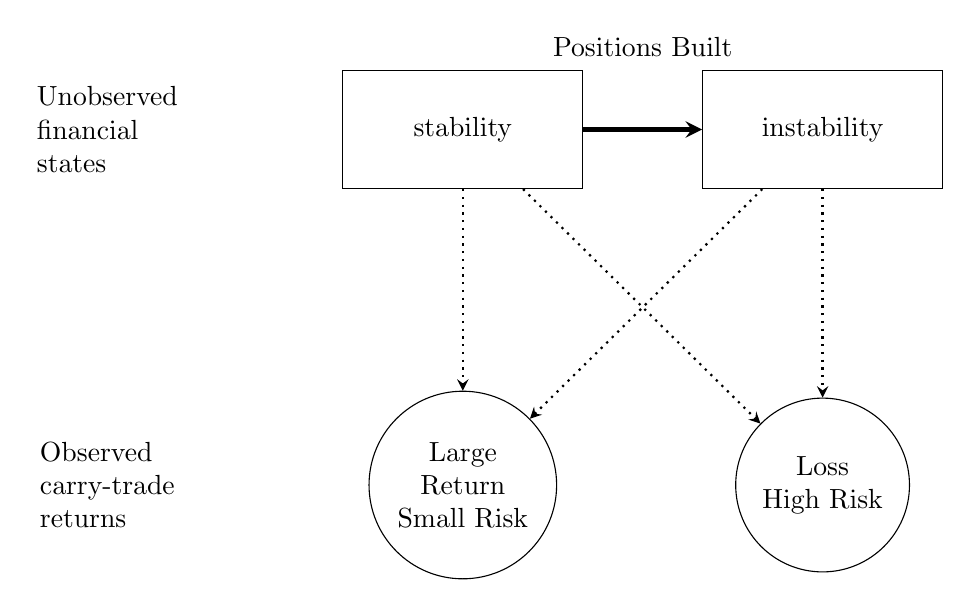
\begin{tikzpicture}
\tikzstyle{decision} = [circle, draw, minimum height = 8mm, 
  text width = 5em, text centered];
\tikzstyle{line} = [draw, -stealth, thick]
\tikzstyle{line2} = [draw, -stealth, ultra thick]
\tikzstyle{line3} = [draw, -stealth, dashed, thick]
\tikzstyle{line4} = [draw, -stealth, dotted, thick]
%\tikzstyle{elli} = [draw, ellipse, fill = red!50, minimum height = 8mm, 
 % text width = 5em, text centered]
\tikzstyle{block} = [draw, rectangle, text width = 8em, 
  text centered, minimum height = 15mm, node distance = 8em]
\node [block](Calm){stability};
%\node [block, left of  = Build, xshift = -5em] (Calm){Calm}; 
\node [block, right  of = Calm, xshift =5em] (Crisis){instability};
\node [decision, below of = Calm, yshift = -10em, align = center]
(Calm2){Large Return \\ Small Risk}; 
\node [decision, below of = Crisis, yshift = -10em](Crisis2) {Loss \\ High Risk};
%\node [decision, below of = Caution, yshift = -10em, align = center](Caution2) 
%{Small \\ Return \\ Average \\ Risk};
%arrows 
%\path [line3] (Calm) -- (Calm);
%\path [line3] (Crisis) -- (Crisis);
%\path [line3] (Crash) -- (Crash2);
\path [line2] (Calm) -- node [yshift = 3em] {Positions Built} (Crisis);
%\path [line2] (Caution) -- node [yshift = 3em]  {Speculative Lending} (Build);
\path [line4] (Calm) -- (Crisis2);
\path [line4] (Crisis) -- (Calm2);
\path [line4] (Calm) -- (Calm2);
\path [line4] (Crisis) -- (Crisis2);
%\path [line4] (Crash) -- (Caution2);
%\path [line4] (Crash) -- (Build2);
\node [align = left, left of = Calm, xshift = -10em] {Unobserved \\ 
financial \\ states};
\node [align = left, left of = Calm2, xshift = -10em] {Observed \\ 
carry-trade\\returns};
%\path [line] (decision1) -| node [yshift = 0.5em, 
%   xshift = 8em] {YES} (process 1);
%\path [line3] (Crash) -- (Caution); 
% 	xshift = -8em] {NO} (process 2);
\end{tikzpicture}
\caption{Two-Regime Hidden Markov Model (HMM)}
\label{figref:HMM2}
\end{figure}
The prior or initial state probabilities give the probability that the system starts in a particular regime; the transition model is the probability of moving from one financial state to another; the response model is the relationship between the observed carry-returns and the unobserved financial regime.  

The starting point of the system is given by,
\begin{equation*}
P(S_1 = 1), \dots P(S_1 = N)
\end{equation*}
as the probability of being in one of $N$ regimes, and the state transition matrix for a two-state system is:

\begin{equation*}
\begin{bmatrix}
P(S_t = 1|S_{t-1}=1)  & P(S_t = 2|S_{t-1}=1)\\
P(S_t = 1|S_{t-1}=2)  & P(S_t = 2|S_{t-1}=2)
\end{bmatrix}
\end{equation*}

  Each element of the matrix shows the probability of being in a particular regime given the previous regime. This is a first-order Markov model.  The transition probabilities depend only on the previous state. This seems to be a reasonable assumption in most circumstances.  However, to assess whether the risk of a financial crisis is increased by the length of the period of stability, it would be necessary to have a higher order Markov chain, increasing the memory of the system and the computational complexity.  In that case an alternative method would be more appropriate. 

\subsection{Estimation of the parameters}
Estimating the HMM involves determining the most likely values for the three sets of parameters in the model.  

\begin{equation}
\lambda = (\pi, A_1, B_1)
\end{equation}

This estimation is done by Maximum Likelihood. As a consequence of the Markov assumption, this is a problem that can be solved with the \emph{Expectation-Maximization (EM) algorithm}.  See \citet{dempster1977maximum} and \citet{Hamilton1989} as well as \citet{depmixS4} for full details of the procedure.  This is a numerical optimisation.  There are two steps. First \emph{the expectation step} will iterate forward from the starting point using prior estimates of the three sets of parameter values  to make an initial assessment of the probability of observing each hidden regime given the model parameters.  The number of regimes is given but whether this is appropriate will be determined using the log-likelihood ratio and other information criteria.  The prior estimates of the parameters can either be drawn randomly or they can be determined by some previous information.\footnote{In this case the parameters are drawn randomly.  However, it would be possible to make initial estimates of the response model from \citet{Hayward2013} using the estimates of the carry-trade returns that are identified.}  In this way the most likely unobserved regime for each period can be calculated. A variant of the EM algorithm called \emph{the forward-backward} or \emph{Baum-Welch} algorithm \citet{Baum1970} is used.   The Baum-Welch algorithm will find the parameters that maximize the probability of observing the sequence of carry-trade returns.  

For the dependent mixture model, the joint likelihood of observation $Y_{1:T}$ and the latent state $S_{1:T}$ given the model parameters is 
\begin{equation}
P(Y_{1:T}, S_{1:T}|\theta) = \pi b_{S_t}(Y_1)\prod_{t-1}^{T-1} a_{i,j}b_{s_t}(Y_{t+1})
\end{equation}

where $\pi_i$ is the initial probability of each state; $a_{i,j} = P(S_{t+1} = j| S_t = i$ is the transition probability; and $b_{S_t}$ is the probability of being in a particular state given the observed carry-trade return, $b_j = P(Y_t|S_t = j)$.

Secondly, the \emph{maximisation step} then updates the most likely values for the three sets of parameters based on the state sequence that has just been identified. Therefore, the probabilities of starting in a particular regime $(\pi)$ come from the estimates just used to assess the most likely regime in each period; the transition matrix $(A)$ is estimated from the given sequence; and the factor weights for the response model $(B)$ are also updated. For the expectations part of the iteration, the states are replaced by their expected value given the parameters of the models $(\mathbf{\theta})$ 

The estimation process then iterates back and forwards between the expectation and maximisation steps until the log-likelihood of the given parameters reaches a peak or the degree of improvement falls below a threshold. It is possible to reach a local maximum so it is usually advisable to run several iterations with different starting values.  That has not been done in this case as a seed has been set for the randomisation process in the interest of reproducibility. 

\section{Analysis of Results}\label{secref:res}
\subsection{Data}
The data to be used are a sample of potential carry-trade investments in CEE countries using a variety of funding currencies that have been compiled from exchange rate and interest rate data for the period from January 2000 to December 2013. The exchange rates are presented in Table \ref{tabref:exrate}.  The data are taken from the IMF International Financial Statistics (IFS).  

\begin{table}[t]
\begin{threeparttable}
\centering
\begin{tabular}{lrr}
  \hline
Country & ISO Code & Exchange rate arrangement\\
  \hline
Bulgaria & BGN & Currency board\\
Czech Republic & CZK & Float\\
Croatia & HRK & Fixed peg\\
Hungary & HUF & Float \\
Poland & PLN & Float\\
Romania & RON & Managed float\\
Russia & RUB & Fixed peg\\
Ukraine & UAH & Managed float\\
Turkey & TRY & Float\\
   \hline
\end{tabular}
\begin{tablenotes}
\small
\item The table shows the exchange rates that are considered with the ISO codes that are used from this point onwards and the exchange rate regime.  The exchange rate regime is taken from the IMF Classification of Exchange Rate Arrangements and Monetary Policy Frameworks \citet{IMFregime}. In many cases there are changes to the arrangements, when that happens the summary here reflects the stance at the end of the period.  For more details see \citet{Hayward2014}.  
\end{tablenotes}
\caption{Countries, ISO codes and exchange rate arrangements}
\label{tabref:exrate}
\end{threeparttable}
\end{table}

The funding currencies are those that have been identified by \citet{FTS}. They are the euro, the US dollar, the Swiss franc and the Japanese yen. A set of potential carry-trade profits are calculated from the exchange rate and interest rate data using a small modification of the method proposed by \citet{BrunnermeierCarry},   

\begin{equation}
p_t = \frac{i^*_t - i_t}{\Delta s_t}
\end{equation} 

where $i_t^*$ is the investment currency, $i_t$ is the funding currency, $\Delta s_t$ is the change in the exchange rate and $p_t$ is the gross profit for potential carry-trades without transaction costs or adjustment for risk.  \citet{Burnside2010} constructs a similar series for a panel of 10 exchange rates and finds a very small effect from plausible transaction costs and Sharpe Ratios that compare favourably with equity markets.  One month and three month positions are calculated. Only the one month are presented as the results do not differ significantly. 

Table \ref{tabref:desst} shows the descriptive statistics for the potential carry-trade profit series. The mean is the annualised potential profits for each country when funded in euro.  Though the monthly Sharpe Ratios are all above one, the significant skews (standing more than two standard errors beyond zero) and the fact that in all cases outside Bulgaria maximum losses outweigh maximum gains is consistent with risk that is not fully captured by conventional measures like standard deviation. The data also suggest that the Czech Republic is a special case and the returns are more normally distributed and there is less skew and kurtosis and this may suggest less of a carry-trade-type currency.  

\begin{sidewaystable}[p]
% latex table generated in R 3.2.3 by xtable 1.8-2 package
% Fri Jun  2 11:56:55 2017
%\begin{table}[t]
\begin{threeparttable}
\centering
\begin{tabular}{lrrrrrrrrrrr}
  \hline
 & HUF & PLN & CZK & RON & RUB & BGN & UAH & HRK & TRY & SPY\\ 
  \hline
Number & 167 & 167 & 167 & 167 & 167 & 167 & 167 & 159 & 166 & 167\\ 
  Mean & 12.80 & 12.41 & 10.07 & 11.94 & 7.21 & 8.09 & 7.84 & 10.73 & 13.56 & 5.19\\ 
  Sharpe & 1.83 & 1.88 & 1.56 & 1.99 & 1.50 & 1.36 & 1.89 & 1.74 & 2.10 & 1.28 \\ 
  Medium & 21.52 & 13.75 & 9.32 & 17.42 & 9.58 & 7.64 & 10.06 & 12.02 & 16.85 & 8.75 \\ 
  StDev & 0.07 & 0.07 & 0.07 & 0.06 & 0.05 & 0.06 & 0.04 & 0.06 & 0.07 & 0.05 \\ 
  Skew & -0.51 & -0.57 & -0.21 & -0.33 & -0.93 & -0.02 & -1.45 & -0.16 & -0.67 & -0.46 \\ 
  SES & 0.19 & 0.19 & 0.19 & 0.19 & 0.19 & 0.19 & 0.19 & 0.19 & 0.19 & 0.19\\ 
  Kurt & 1.64 & 1.40 & 0.44 & 1.36 & 3.37 & 1.02 & 7.37 & 0.90 & 2.60 & 0.66\\ 
  SEK & 0.99 & 0.99 & 0.99 & 0.99 & 0.99 & 0.99 & 0.99 & 0.99 & 0.99 & 0.99\\ 
  Max & 20.41 & 18.61 & 18.09 & 17.26 & 16.02 & 21.58 & 14.76 & 17.66 & 18.64 & 11.49\\ 
  Min & -25.49 & -21.84 & -19.56 & -20.75 & -21.11 & -18.88 & -21.93 & -19.03 & -26.68 & -16.04\\ 
   \hline
\end{tabular}
\begin{tablenotes}
\small 
\item The table shows the descriptive statistics for the calculated potential carry-trade profits for each country plus a comparison with the S\&P 500. Number is the number of observations; Mean is the annualised return; Sharpe is the monthly Sharpe Ratio, assuming a risk-free rate of zero; Median is the median annualised return; StDev is the standard deviation; Skew is the measure of Skewness of the distribution; SES is the standard error of skewness so that a skewness that is twice this size could be considered to be statistically significant at the 5\% level; Kurt is the measure of excess kurtosis; SEK is the standard error of kurtosis; Max is the maximum return; Min is the minimum return. 
\end{tablenotes}
\caption{Descriptive statistics of potential carry-trade profits}
\label{tabref:desst}
\end{threeparttable}
%\end{table}
\end{sidewaystable}

\subsection{Model Comparison}
Initially, there are three models that are applied to each of the carry-trade-profit series. 
\begin{itemize}
\item Model One (M1) is a standard linear model $p_t = \beta_0  + \varepsilon_t$ where $p_t$ is the carry-trade-profit series, $\beta_0$ is the intercept and $\varepsilon_t$ is the variation around that level.  It provides a mean and standard deviation for the potential carry-trade-profit for the whole period.  These are the figures presented in Table \ref{tabref:desst}.
\item Model Two (M2) is a standard linear model with two regimes $p_t = \beta_0 + \beta_1 S_n + \varepsilon, \quad n = 1, 2$ therefore a mean and a standard deviation of the potential carry-trade profits for each of the two regimes is produced.  The mean and standard deviation of the potential carry-trade profits for each regime are presented in Table \ref{tabref:2stateresponse}.
\item Model Three (M3) is a standard linear model with three regimes $p_t = \beta_0 + \beta_1 S_n + \varepsilon, \quad n = 1, 2, 3$ average and standard deviations are retrieved for three different regimes. 
\end{itemize}

The models are compared using the Akaike Information Criterion (AIC) and the log-likelihood ratios (LLR) adjusted for the number of parameters estimated.  Table \ref{tabref:comptab2} summarises the performance of the three base models using these criteria. The models here are tested using the euro as the funding currency.  Results for other funding currencies are very similar and are therefore not reported.  A comparison of the mean and variance for the two-regime response models for different funding units is presented in Table \ref{tabref:2stateresponse}. 

\begin{sidewaystable}[p]
% latex table generated in R 3.0.2 by xtable 1.7-1 package
% Mon Aug 18 09:06:42 2014
%\begin{table}[ht]
\begin{threeparttable}
\centering
\begin{tabular}{l|rrrrrrrrrr}
  \hline
 & AIC(M1) & ACI(M2) & AIC(M3) & LLR21 & LLR21p & LLR31 & LLR31p & LLR32 & LLR32p & Preferred\\ 
  \hline HUF & -404.69 & -416.94 & -407.23 & 22.25 & 0.0005 & 26.50 & 0.0090 & 4.30 & 0.7459 & M2\\  PLN & -423.98 & -437.62 & -428.82 & 23.65 & 0.0003 & 28.80 & 0.0042 & 5.20 & 0.6357 & M2\\  CZK & -427.23 & -427.37 & -415.61 & 10.14 & 0.0714 & 12.40 & 0.4155 & 2.20 & 0.9451 & M1 or M2\\  RON & -456.02 & -474.81 & -464.39 & 28.79 & 0.0000 & 32.40 & 0.0012 & 3.60 & 0.8264 & M2\\  RUB & -523.18 & -567.77 & -559.95 & 54.59 & 0.0000 & 60.80 & 0.0000 & 6.20 & 0.5188 & M2\\  BGN & -451.98 & -454.32 & -443.21 & 12.34 & 0.0305 & 15.20 & 0.2291 & 2.90 & 0.8945 & M2\\  UAH & -572.87 & -643.36 & -636.39 & 80.49 & 0.0000 & 87.50 & 0.0000 & 7.00 & 0.4257 & M2\\ 
  HRK & -431.55 & -433.37 & -426.58 & 11.82 & 0.0373 & 19.00 & 0.0877 & 7.20 & 0.4068 & M2\\ 
  TRY & -431.05 & -441.00 & -432.58 & 19.95 & 0.0013 & 25.50 & 0.0125 & 5.60 & 0.5895 & M2\\ 
   \hline
\end{tabular}
\begin{tablenotes}
\small
\item Three models are initially tested.  Model One (M1) is the base model with carry-trade returns explained by a normal distribution around a linear constant; Model Two (M2) is the linear model with 2 regimes; Model Three (M3) is the linear model with 3 regimes.  AIC measures the Akaike Information index for the model identified, LLR is the log-likelihood ratio test statistics that compares the two named and nested models.  The p indicates the probability value of the $\chi^2$ test of the log-likelihood ratio with degrees of freedom equal to the number of parameter constraints of the base model.  For example LLR32p is the probability value for the ratio between Model Three (M3) and Model Two (M2).
\end{tablenotes}
\caption{Comparison of models}
\label{tabref:comptab2}
\end{threeparttable}
%\end{table} 
\end{sidewaystable}

Table \ref{tabref:comptab2} compares the three fundamental models with 1, 2 and 3 regimes respectively.  The aim is to find the number of regimes that provide the best fit for each of the potential carry-trade profit series for each country.  In each case the test is based on the requirement that the log-likelihood ratio improve by more than would be expected with the increase in the number of explanatory variables.  The first three columns of Table \ref{tabref:comptab2} report the AIC for each of the three base models respectively. The next six columns show the Log-likelihood ratio test statistic and the p-value for a comparison of Model One (M1) to Model Two (M2), Model One (M1) to Model Three (M3) and Model (M2) to Model Three (M3) respectively. The null is that the more sophisticated or complex model (two regime rather than one for example) does not improve the explanatory power by more than would be expected with the additional variables. The final column combines the two tests to present the model that appears to fit the data most effectively. 

The two-regime model is superior to the base model with one regime for all countries.  However, for the Czech Republic there is ambiguity.  For the Czech Republic, the null of no-improvement can be rejected at the 10\% level but not the 5\%.  The Czech Republic may be better assessed with just a single regime. This case will be investigated further below. 

Table \ref{tabref:2stateresponse} presents the estimated response (mean and standard deviation) for each of the two-regimes models. The results are encouraging for the hypothesis that potential carry-trade profits are best modelled as two regimes where one of them is considered the period of calm where carry positions are build and the other is considered the period of crisis where carry-trade positions will be cut back.  In the first case, the the ratio $p_t$ should be above one.  This is consistent with the estimated value of $\beta_1$ in Equation \ref{eq:uip2} being below one.  The period labelled calm should also be expected to have smaller standard deviation and less risk because exchange rate conditions are expected to be calm when carry-trade positions can be built.  The crisis period should have a mean of less than one and a larger standard deviation to reflect the increased risk that is being taken in this regime. This is when the crash risk happens.  The mean and standard deviation for the two regimes are those that are most appropriate for the data.  It is certainly possible that the regime with the lower mean could also have the smallest standard deviation.  However, this does not happen in any of the cases. 

There are two other things to note.  First, the funding currency that is selected does not make much difference.   In no case does the basic result change when different funding currencies are applied. As a consequence, the rest of the results that are presented are based on euro-funding.  Secondly, the results for the Czech Republic support the view that one regime may be a better way to model the data. Though two regimes can be estimated, the distribution of the potential carry-trade profits does not differ much between the two. 

\begin{sidewaystable}[p]
% latex table generated in R 3.0.2 by xtable 1.7-1 package
% Sat Jul 12 08:23:47 2014
%\begin{table}[ht]
\begin{threeparttable}
\centering
\begin{tabular}{llrrrrrrrrrrr}
  \hline
 Funding & Regime& & HUF & PLN & CZK & RON & RUB & TRY & BGN & UAH & HRK & Mean \\ 
  \hline
  \hline
\multirow{4}{*}{EUR}& \multirow{2}{*}{Stable}& Mean & 1.0165 & 1.0173 & 1.0129 & 1.0150 & 1.0098 & 1.0151 & 1.0075 & 1.0094 & 1.0091 & 1.0119 \\ 
&&St-Dev& 0.0519 & 0.0486 & 0.0542 & 0.0433 & 0.0310 & 0.0460 & 0.0381 & 0.0295 & 0.0251 & 0.0446 \\ 
&\multirow{2}{*}{Crash}& Mean & 0.9905 & 0.9862 & 0.9963 & 0.9969 & 0.9962 & 0.9969 & 1.0053 & 0.9673 & 1.0082 & 0.9897 \\ 
 &&S-Dev & 0.1085 & 0.1026 & 0.0886 & 0.0878 & 0.0779 & 0.1028 & 0.0826 & 0.1116 & 0.0737 & 0.0958 \\ 
\hline
\multirow{4}{*}{USD}&\multirow{2}{*}{Stable}&Mean& 1.0103 & 1.0123 & 1.0072 & 1.0091 & 1.0044 & 1.0087 & 1.0041 & 1.0055 & 1.0054 & 1.0071 \\ 
&&S-Dev& 0.0307 & 0.0297 & 0.0305 & 0.0080 & 0.0095 & 0.0314 & 0.0189 & 0.0078 & 0.0187 & 0.0202 \\ 
  &\multirow{2}{*}{Crash}&Mean& 0.9925 & 0.9845 & 0.9983 & 1.0052 & 1.0004 & 1.0034 & 1.0016 & 0.9932 & 1.0036 & 0.9959 \\ 
   & & S-Dev & 0.0707 & 0.0641 & 0.0493 & 0.0389 & 0.0407 & 0.0792 & 0.0413 & 0.0635 & 0.0390 & 0.0566 \\ 
\hline
\multirow{4}{*}{CHF}& \multirow{2}{*}{Stable}&Mean& 1.0052 & 1.0097 & 1.0040 & 1.0085 & 1.0033 & 1.0099 & 1.0012 & 1.0029 & 1.0031 & 1.0051 \\ 
   & & S-Dev & 0.0181 & 0.0235 & 0.0161 & 0.0179 & 0.0234 & 0.0313 & 0.0083 & 0.0307 & 0.0116 & 0.0205 \\ 
   & \multirow{2}{*}{Crash}& Mean & 0.9994 & 0.9838 & 0.9934 & 0.9959 & 0.9373 & 0.9952 & 0.9958 & 0.9834 & 0.9916 & 0.9857 \\ 
  & & S-Dev & 0.0477 & 0.0459 & 0.0380 & 0.0387 & 0.0592 & 0.0792 & 0.0327 & 0.0900 & 0.0384 & 0.0538 \\ 
\hline  
  \multirow{4}{*}{JPY}&\multirow{2}{*}{Stable}& Mean& 1.0149 & 1.0157 & 1.0125 & 1.0149 & 1.0074 & 1.0111 & 1.0092 & 1.0094 & 1.0091 & 1.0115 \\ 
 & & S-Dev &0.0348 & 0.0359 & 0.0241 & 0.0291 & 0.0226 & 0.0401 & 0.0191 & 0.0307 & 0.0210 & 0.0289 \\ 
  & \multirow{2}{*}{Crash}&Mean & 0.9843 & 0.9727 & 1.0012 & 0.9972 & 0.9983 & 1.0061 & 1.0002 & 0.8539 & 1.0028 & 0.9801 \\ 
  & & S-Dev& 0.0767 & 0.0764 & 0.0525 & 0.0580 & 0.0628 & 0.0889 & 0.0487 & 0.0667 & 0.0493 & 0.0668 \\ 
   \hline
\end{tabular}
\begin{tablenotes}
\small
\item
This table outlines the linear response for Model Two (M2) for each of the regimes for all countries under consideration.  Stable is the label given to the regime with the highest mean return.  In all cases this is also the regime with the smallest standard deviation. This is not imposed and it is encouraging as, consistent with the idea that the carry-trade is composed of two distinct phases, it suggests that positions are built and profits are available when conditions are stable and that losses are suffered when conditions are more risky.  Figures for the Czech Republic should be treated with some caution.  The data also suggests that the funding currency does not have a major effect on the performance of the carry-trade.   
\end{tablenotes}
\caption{Mean and Standard Deviation of 2 Regime Model}
\label{tabref:2stateresponse}
\end{threeparttable}
%\end{table}
  \end{sidewaystable}

The other interesting issue is the transition matrix that determines the probability of switching from one regime to another. The most important of these elements is the probability that a period of stability or calm will move to one of crisis.  The other item of interest is how likely it is that the crisis persists once it starts\footnote{The other two components (remaining in the calm regime and switching from a period of crisis to one of calm) can be calculated from these transition probabilities.}  Table \ref{tabref:transprob} provides these figures.  The probability that a period of calm will turn into a period of crisis ranges from just one percent in the Czech Republic to as much as fifty percent in Croatia. Once a crisis has stated it persists for a while. In all cases this is estimated at between seventy five and ninety five percent.

\begin{table}[t]
\begin{threeparttable}
\centering
\begin{tabular}{p{3cm}rrrrrrrr}
  \hline
& CZK & HRK & HUF & PLN & RON & RUB & TRY & UAH\\ 
  \hline
Calm to Crisis & 0.01 & 0.50 & 0.04 & 0.04 & 0.01 & 0.01 & 0.10 & 0.01\\
Remain in Crisis & 0.97 & 0.74 & 0.88 & 0.87 & 0.97 & 0.98 & 0.71 & 0.91 \\
  \hline
\end{tabular}
\begin{tablenotes}
\small
\item  The table shows the transition probabilities for each of the countries.  The first row records the probability that a calm regime will switch to one of currency crisis; the second row shows the probability that once in the regime of currency crisis, the regime will remain in place. 
\end{tablenotes}
\caption{Transition probabilities}
\label{tabref:transprob}
\end{threeparttable}
\end{table}

It is also possible to look at the evolution of most likely regimes over time.  Figure \ref{figref:pln} shows the potential carry-trade profits and the two regimes for Poland.  It is clear that the Global Financial Crisis (GFC) is the main regime change that takes place.  Not surprisingly, this episode dominates the data.  This probably explains the persistence of the crisis once it starts. There are also a number of smaller mini-crises that are also evident in the turmoil after the GFC. 

\begin{figure}[ht]
\centering
\includegraphics[scale = .50]{../../Figures/PLNEUR2.pdf}
\caption{PLN Carry-trade probabilities}
\label{figref:pln}
\end{figure}

\section{Exogenous influences on regime switching probabilities}
Periods of foreign exchange crisis are generally referred to as \emph{sudden stops}.  See \citet{DornbuschSS}, \citet{CalvoSS} and \citet{KrugmanSS} for more details. Calvo  defines the sudden stop as net capital flows moving two standard deviations below their mean level and subsequently returning to within one standard deviation of that point. There are a number of factors that may influence capital flows and exchange rate stability. Exchange rate crisis can be caused by domestic or international factors.  \citet{FTS} find  that exogenous factors that cause sudden stops and flight-to-safety of \emph{hard} currencies  are relatively rare events. Their study of of 23 countries finds that most of the events are country specific. They characterise only 25\% of the events as \emph{global}. However, it is the exogenous international effects that are the focus here and these are the cases where a global increase in risk aversion cases a capital retreat from emerging economies and a shift towards what are perceived to be safe and stable assets. 

  Consistent with the evidence of an interplay between monetary policy and international risk, and between domestic and international factors, \citet{Ahmed2014} show that economic growth, interest rate differentials and the level of global risk appetite are all important determinants of private capital flows to emerging markets.  They also suggest that capital flows have been more sensitive to interest rate differentials since the financial crisis of 2007-08. There is also some evidence that US quantitative easing has affected capital flows to emerging economies.  Funds flow from the US Federal Reserve into high yielding assets in emerging economies. 

\citet{NYFedtaper} consider the effect of changes in global risk aversion on the carry-trade.  They find that the initial signal from the US central bank in Fed Chairman Bernanke's May 22 2013 testimony to Congress coincide with an increase in global risk aversion which affected global asset prices.  By identifying the performance of exchange rates without a change in risk aversion, they suggest that nearly half of the depreciation of a basket of 45 carry-trade currencies with the largest one-month interest rate relative to a basket of the US dollar and other equally low rate currencies is explained by this increased risk aversion. Nearly all the decline in Emerging market equities is attributable to the increase in risk aversion.

\citet{IMFLatam} use a panel vector autoregression (VAR) method to identify the influence of US monetary policy since 1990 on capital flows to 38 emerging economies, finding evidence that the end to Federal Reserve purchase of government bonds under the quantitative easing programme, while not necessarily leading to capital outflow, could generate \emph{new risk premium shocks} with investors requiring a higher rate of return and therefore lower asset prices.

\subsection{Additional Models}
This section will examine whether exogenous factors influence the potential profitability of the carry-trade or the probability of switching from a regime of foreign exchange calm to one of crisis.  The two exogenous forces are to be tested are international risk aversion and US interest rates.  Risk aversion is measured with the VIX index while US interest rate are measured as the 3-month US dollar deposit\footnote{The VIX is an index of implied volatility on options from the S\&P 500 index.  It is commonly used as a measure of international risk aversion as it signals increased demand by fund managers for option protection of their equity portfolio.  See \citet{VIX}, \citet{GoldmanVol} and \citet{Diamond} for fuller details.}.   

These external forces could affect foreign exchange conditions and the carry-trade in two ways:  they could have a direct linear influence on rates or they could influence the probability of switching from one regime to another.  In the first case they could be added as an explanatory variable to the simple linear response model. For example, 

\begin{equation}
\label{eqref:vix}
y_t = \beta_0 + \beta_1 Z_t + \varepsilon
\end{equation}

where $y_t$ is the carry-trade return and $Z_t$ is the exogenous influence on financial stability (either international risk aversion or US interest rates). This is Model Four (M4) with two versions a and b to signify the effect of risk aversion and US interest rates respectively.  

In the second case, the exogenous force may influence the transition probabilities using a multinomial logistic regression. For the transition model (A), 

\begin{equation}
a_{ij}(t) = P(S_t = j|S_{t-1} = i, z)
\end{equation}

where $a_{ij}(t)$ is the probability that the system will be in state $i$ at time $t$ when it was in state $j$ in the previous period and  covariate $z$ takes a particular value at time $t$.  For a two-regime model, the  estimation that is carried out is 

\begin{equation}
log(a_{t,n = 2})/ a_{t-1, n = 1} = \beta_{0} +\beta_1 z_t 
\end{equation}

State 1 is the baseline category so coefficients are set to zero for that state and the model estimates the relationship between the covariate and probability of switching to the other state. 

The logistic function used for this is 
\begin{equation} 
F(z)  = \frac{1}{1 + e^{-(\beta_0 + \beta_1 z)}}
\label{eqref:zcov}
\end{equation}
 
giving the estimated probability of being in the particular state conditional on having been in a particular state in the previous period and conditional on the exogenous variable being at a particular level.  See \citet[pp.174-75]{agresti2014categorical} for more details.  This is Model Five (M5). There are also two version of this model (a and b) that will denote whether the probability of switching from one state to the other is conditional on risk aversion or US interest rates. 

\begin{sidewaystable}[p]
% latex table generated in R 3.0.2 by xtable 1.7-1 package
% Fri Aug 22 12:24:06 2014
%\begin{table}[]
\begin{threeparttable}
\centering
\begin{tabular}{rrrrrrrrrrrr}
  \hline
 & AIC(M1) & ACI(M4) & AIC(M2) & AIC(M5) & LLR54 & LLR54p & LLR52 & LLR52p & Coeff & p-value & Preferred\\ 
  \hline
HUF & -404.69 & -402.70 & -416.94 & -419.50 & 28.80 & 0.0001 & 6.56 & 0.0377 & -0.00 & 0.9529 & M5\\ 
  PLN & -423.98 & -422.03 & -437.62 & -438.93 & 28.90 & 0.0001 & 5.30 & 0.0705 & -0.00 & 0.8202 & M5/2\\ 
  CZK & -427.23 & -425.25 & -427.37 & -430.52 & 17.27 & 0.0083 & 7.15 & 0.0280 & 0.00 & 0.8935 & M5\\ 
  RON & -456.02 & -454.42 & -474.81 & -478.07 & 35.65 & 0.0000 & 7.26 & 0.0265 & 0.00 & 0.5307 & M5\\ 
  RUB & -523.18 & -449.98 & -567.77 & -566.68 & 128.70 & 0.0000 & 2.92 & 0.2328 & -0.00 & 0.9833 & M2\\ 
  BGN & -451.98 & -449.98 & -454.32 & -459.55 & 21.56 & 0.0015 & 9.23 & 0.0099 & -0.00 & 0.9892 & M5\\ 
  UAH & -572.87 & -571.47 & -643.36 & -647.67 & 88.20 & 0.0000 & 8.31 & 0.0157 & 0.00 & 0.4451 & M5\\ 
  HRK & -431.55 & -429.58 & -433.37 & -439.42 & 21.84 & 0.0013 & 10.05 & 0.0066 & -0.00 & 0.8590 & M5\\ 
  TRY & -431.05 & -429.06 & -441.00 & -439.26 & 22.20 & 0.0011 & 2.26 & 0.3232 & -0.00 & 0.9575 & M2\\ 
   \hline
\end{tabular}
\begin{tablenotes}
\small
\item The table details the comparison of four models. Here Model  One (M1) is the base model; Model Four (M4a) adds the VIX index as a response variable (Equation \ref{eqref:vix}); Model Two (M2) is the simple response model with two regimes; Model Five (M5a) is the two-regime model with the VIX index providing a logistic covariate of the transition matrix. LLR is the log-likelihood ratio with the p denoting the p-value for a $\chi^2$ distribution with degrees of freedom equal to the parameter restrictions on the base model that is being compared.  Therefore, LLR54p is the p-value for the log-likelihood ratio of Model Five on Model Four.  This assesses the performance of the two-regime model with the VIX influencing the transition values against the model where the VIX directly affects the carry-trade return. Coefficient is from Model Four.  It is the estimate of $\beta_1$ from a regression of Equation \ref{eqref:vix}; p-value is the test of the null hypothesis that $\beta_1$ is equal to zero. 
\end{tablenotes}
\caption{VIX covariate model table}
\label{tabref:vixcov}
\end{threeparttable}
%\end{table}
\end{sidewaystable}

Table \ref{tabref:vixcov} compares models M4a and M5a against models M1 and M2.  Models 4a and 5a use the VIX as a measure of international risk aversion as with an explanatory variable (M4a Equation \ref{eqref:vix}) or as conditioning for the transition probability matrix (M5a Equation \ref{eqref:zcov}).  Model One (M1) the base model with one state and a linear relationship. There are three criteria used to judge the preferred model: the AIC, log-likelihood ratios and simple linear regression of the additional exogenous explanatory variable. Columns 1 to 4 report the AIC for the M1, M4a, M2 and M5a models respectively.  Columns 5 and 6 report respectively the log likelihood ratio test statistic and the p-value for Model 5a relative to Model 4a; Columns 7 and 8 do the same for the comparison of Model 5a over Model 2.  Columns 9 and 10 report the t-statistic and p-value of a line regression of the potential carry-trade profits on a constant and the VIX index and the p-value. This is Equation \ref{eqref:vix} and the estimate is $\beta_1$.  Column 11 identifies the model that is most appropriate for each series according to these criteria.

Model 5 is the preferred model in most cases.  For Poland, there is a little uncertainty about whether Model Two or Model Five is better.  As we shall seen, this is because exogenous factors do not have a major influence on Poland. For Russia and Turkey, while it appears that the level of international risk aversion is best used explaining the probability of switching from one regime to another rather than as an explanation of the level of carry-trade profits, it also appears that the simple two-regime model provides the best fit.

%\begin{landscape}
% latex table generated in R 3.0.2 by xtable 1.7-1 package
% Fri Aug 22 14:23:21 2014
\begin{table}[t]
\begin{threeparttable}
\centering
\begin{tabular}{rrrrrrrr}
  \hline
 & -3sd & -2sd & -1sd & Mean & +1sd & +2sd & +3sd \\ 
  \hline
  HUF & 0.0020 & 0.0069 & 0.0242 & 0.0807 & 0.2375 & 0.5249 & 0.7967 \\ 
  PLN & 0.0004 & 0.0016 & 0.0063 & 0.0242 & 0.0887 & 0.2766 & 0.6003 \\ 
  CZK & 0.0020 & 0.0062 & 0.0234 & 0.0770 & 0.2247 & 0.5019 & 0.7779 \\ 
  RON & 0.0014 & 0.0043 & 0.0131 & 0.0392 & 0.1119 & 0.2799 & 0.5453 \\ 
  RUB & 0.0008 & 0.0022 & 0.0065 & 0.0189 & 0.0537 & 0.1430 & 0.3291 \\
  BGN & 0.0052 & 0.0145 & 0.0403 & 0.1066 & 0.2533 & 0.4910 & 0.7328 \\ 
  HRK & 0.0027 & 0.0073 & 0.0194 & 0.0506 & 0.1257 & 0.2793 & 0.5109 \\ 
   \hline
\end{tabular}
\begin{tablenotes}
\small
\item Changes in the VIX index affect the transition probabilities.  The VIX index has been scaled so that it has a mean of zero and a standard deviation of one.  Therefore, the central column shows the probability that the system will switch from a stable regime to one of crisis when the VIX is at its average level.  It also shows how this probability changes as the VIX moves one or more standard deviations above and below this average. For example, for Hungary, there is an 8\% chance that the system will switch to a period of crash when the VIX is at its average value.  This rises to 24\% when the VIX is one standard deviation above average and 52\% for 2 standard deviations.  
\end{tablenotes}
\caption{Assessing the influence of VIX index on financial risk} 
\label{tabref:vixtranprob}
\end{threeparttable}
\end{table}

Table \ref{tabref:vixtranprob} provides more detail about Model 5.  The changes in the VIX index are normalised to one standard deviation and the base probability of moving from the calm regime when there there is a good chance of achieving carry-trade profits to one of foreign exchange crisis is recorded at various levels of international risk aversion.  The average level of international risk aversion (as record by the VIX index) is the central column labelled \emph{Mean}.  The probability of switching from a regime of calm to one of crisis is then recorded for one, two and three standard deviations above and below this mean.  These are in columns 6, 7 and 8, and 2, 3 and 4 respectively.  For example, for HUF, there is an eight percent  probability of switching from a period of calm to a period of crisis when the VIX is at its average level. This increases to just under twenty-four percent when the VIX is one standard deviation above the mean and reaches nearly eighty percent at three standard deviations above the mean. 

Table \ref{tabref:vixcov} also gives the best overview of the effect of international factors on the possibility of a financial crisis.  The central column shows that when risk aversion is at an average level the probability of a crash will range from about 8\% in Hungary to around 2\% in Poland and Romania.  The 8\% reading for Czech, considered one of the pillars of stability in the region is a little surprising. We have already noted that the Czech Republic appears to be a special case. This is probably a function of the analysis ending in 2013.  The probability of facing a financial shock increases quite sharply as international risk aversion rises above its average level: at two standard deviations, it is suggested that there is a 50\% chance of a financial shock in Hungary and the Czech Republic (again surprising) and a 28\% chance in Poland, Romania and Croatia. 

% latex table generated in R 3.0.2 by xtable 1.7-1 package
% Fri Aug 22 14:23:21 2014
\begin{table}[t]
\begin{threeparttable}
\centering
\begin{tabular}{rrrrrrrr}
  \hline
 & -3sd & -2sd & -1sd & Mean & +1sd & +2sd & +3sd \\ 
  \hline
  PLN & 0.6601 & 0.4110 & 0.2005 & 0.0827 & 0.0314 & 0.0115 & 0.0042 \\
  RON & 0.0062 & 0.0106 & 0.0182 & 0.0310 & 0.0524 & 0.0871 & 0.1414 \\ 
  RUB & 0.0011 & 0.0025 & 0.0056 & 0.0126 & 0.0283 & 0.0620 & 0.1305 \\
   \hline
\end{tabular}
\begin{tablenotes}
\small
\item Changes in US 1-month interest rates affect the transition probabilities.  The US 1-month interest rate has been scaled so that it has a mean of zero and a standard deviation of one.  Therefore, the central column shows the probability that the system will switch from a stable regime to one of crisis when the 1-month interest rate is at its average level.  It also shows how this probability changes are the 1-month interest rate moves one or more standard deviations above and below this average. For example, for Romania there is a three percent chance of moving to a foreign exchange crisis when US interest rates are at their mean level.  This rises to five, nine and fifteen percent as interest rates move one, two and three standard deviations above average. .  
\end{tablenotes}
\caption{Assessing the influence of US 1-month interest rate on financial risk} 
\label{tabref:1mtranprob}
\end{threeparttable}
\end{table}

Table \ref{tabref:1mtranprob} shows the conditional-transition model that is based on 1-month US interest rates.  There are only a few countries where the model works.  With Poland, the results are contrary to expectations.  As US interest rates move above average levels the risk of moving from a calm to crisis exchange rate regime is reduced.  This is probably a result of the limited span of data that is available, the fact that US interest rates were generally falling in the period and the fact that US rate cuts often follow a international financial crisis.  Romania and Russian are more conventional and show modest positive effects from increased US interest rates on the risk of suffering a financial shock.

A similar analysis was carried out with the TED spread. This is the spread between tbills and eurodollar rates and is used to capture banking credit risk.  There is no case where the TED spread provides any improvement in the standard two-regime model.  Again, the failure may be a consequence of the limited data span. There is just one episode where there was a significant increase in the spread (around the time of the Lehman Brothers' bankruptcy in October 2008 where the spread reached 335bp).

\section{Conclusions}\label{secred:con}
In this paper we have looked at the way that the carry-trade can be modelled as a two-regime system that switches from what can be called a period of calm to one of crisis with a simple Markov model.  In all the cases assessed here the two-regime model provides a better fit for the data than a model with either one or three regimes. We identify the risk that each country will move from a position of calm to one of crisis. We also show that the probability of switching from a period of calm to a period of crisis is affected by exogenous factors like the level of international risk aversion.  

The method can be used to assess country risk and the contribution of various factors (such as exchange rate regime) to the risk.  This way of looking at the UIP puzzle also adds to the evidence that the returns to the carry trade are at least partly a compensation for taking crash-risk.  The breakdown in UIP only holds during the regime that can be described as calm.  In the other regime, there is a risk of large losses that can potentially overwhelm all the gains that were achieved during the period of calm. 

The use of the first-order Markov model does mean that there is a short memory and the time spent in a condition of calm does not affect the probability of a crisis.  However, it is still possible that more time that the system has been stable could have consequences for the size of the shock that is experienced. In that case it may be that a larger dataset could identify three regimes with the final one being a true shock that only happens in extreme rare cases. 

The study of CEE countries is affected by the relative lack of data and the importance of the GFC.  Extending the examination to assess the way that external factors can influence the probability of switching from a period of calm to one of crisis reveals some unusual results.  External factors do not seem to have a major influence on the probability of switching to an unstable foreign exchange regime in Poland.    This seems to be a consequence of the modest reaction to the  GFC.  The greater vulnerability of the Czech Republic is surprising but throughout this process it appears that the two-regime model does less well in explaining potential carry-trade profits in for the Czech exchange rate and this may be because in recent years the CZK has been less of a traditional carry-trade currency. 

%Many studies look at the carry-trade in a mechanical way to borrow the low interest rate currency and invest in that which has a higher r (see for example \citet{Jurek2} and \citet{Elliot}.  See for example \citet{Jurek2} and \citet{Elliot}.  However, in general, there much more likely to be a carry-trade where there is a substantial and sustained interest rate differential. This means that it is more likely to direct funds to emerging economies.  The exchange rates of developing economies are much more likely to suffer liquidity shocks and major depreciations.  The crash risk here likely to be more pronounced and threatening than that of developed economy exchange rates. 
%We have shown that a financial crisis that is caused by a \emph{sudden-stop} can be modelled as a two-regime system and we have estimated the probability that the system will switch from calm to crisis.  The two regimes are identified by the performance of a carry-trade.  When this is successful and profits are being generated, the system is in a state of calm and investors are able to take advantage of the break-down in uncovered-interest-parity (UIP).  However, when the carry-trade starts to lose money as a result of the depreciation of the investment currency relative to the funding, a self-fulfilling crisis is invoked by the attempt to exit the trade.  

%In most of the cases studied here, the two-regime model is superior to the three-regime or one-regime model. However, the modelling is affected by the relatively short time span that has existed since the breakup of the Soviet Union and the establishment of independent countries and currencies.  The attempt to identify how international financial factors affect the probability that a country will switch from a state of calm to one of financial crisis is hindered by the lack of data that this short time span ensures.  While the measurement used for international risk aversion (the VIX index) has sufficient volatility to allow identification, the use of US interest rates and measures of banking system vulnerability are less successful.  It appears that in these cases, there are insufficient examples of rising interest rates or higher banking risk premia to allow relationships to be successfully identified.  


%Maximise $P(O \lambda)$, where $\lambda = (\pi, A, B)$.  The probability of observing sequence O for a given set of parameters.  The easiest way of doing this is to calculate the probability for each of the possible state sequences.  Consider one such sequence, $Q = q_1 q_2 \dots q_T$, the probability of the observed sequence for the state sequence Q is $P(O|Q \lambda) = \prod_{t = 1}^T P(O_t|q_t, \lambda)$.  If the observations are independent, this probability $P(O|Q \lambda)$ is equal to the probability of observing the outcome given the state, $b_{q_1}(O_1)\dot b_{q_2} (O_2) \dots b_{q_T}(O_T)$.  At each step, the forward variable $\alpha_t(i) = P(O_1 O_2 \dots O_t, q_t = S_i|\lambda)$ is calculated as the product of the sum of all the probability of each state for the previous period and the probability of transition from each of those states to the current as well as the product of being in this state given the observable. $\alpha_t(i)$ is the joint probability that observation is seen and state is achieved. 

\bibliography{../../../myrefs}



\end{document}
